\documentclass[man]{apa6}
\usepackage{lmodern}
\usepackage{amssymb,amsmath}
\usepackage{ifxetex,ifluatex}
\usepackage{fixltx2e} % provides \textsubscript
\ifnum 0\ifxetex 1\fi\ifluatex 1\fi=0 % if pdftex
  \usepackage[T1]{fontenc}
  \usepackage[utf8]{inputenc}
\else % if luatex or xelatex
  \ifxetex
    \usepackage{mathspec}
  \else
    \usepackage{fontspec}
  \fi
  \defaultfontfeatures{Ligatures=TeX,Scale=MatchLowercase}
\fi
% use upquote if available, for straight quotes in verbatim environments
\IfFileExists{upquote.sty}{\usepackage{upquote}}{}
% use microtype if available
\IfFileExists{microtype.sty}{%
\usepackage{microtype}
\UseMicrotypeSet[protrusion]{basicmath} % disable protrusion for tt fonts
}{}
\usepackage{hyperref}
\hypersetup{unicode=true,
            pdftitle={Lab 8},
            pdfauthor={Teresa Chen, Jun Lun, Steffi Hung, \& Ting-fen Lin},
            pdfkeywords={math, reading, free lunch},
            pdfborder={0 0 0},
            breaklinks=true}
\urlstyle{same}  % don't use monospace font for urls
\usepackage{graphicx,grffile}
\makeatletter
\def\maxwidth{\ifdim\Gin@nat@width>\linewidth\linewidth\else\Gin@nat@width\fi}
\def\maxheight{\ifdim\Gin@nat@height>\textheight\textheight\else\Gin@nat@height\fi}
\makeatother
% Scale images if necessary, so that they will not overflow the page
% margins by default, and it is still possible to overwrite the defaults
% using explicit options in \includegraphics[width, height, ...]{}
\setkeys{Gin}{width=\maxwidth,height=\maxheight,keepaspectratio}
\IfFileExists{parskip.sty}{%
\usepackage{parskip}
}{% else
\setlength{\parindent}{0pt}
\setlength{\parskip}{6pt plus 2pt minus 1pt}
}
\setlength{\emergencystretch}{3em}  % prevent overfull lines
\providecommand{\tightlist}{%
  \setlength{\itemsep}{0pt}\setlength{\parskip}{0pt}}
\setcounter{secnumdepth}{0}
% Redefines (sub)paragraphs to behave more like sections
\ifx\paragraph\undefined\else
\let\oldparagraph\paragraph
\renewcommand{\paragraph}[1]{\oldparagraph{#1}\mbox{}}
\fi
\ifx\subparagraph\undefined\else
\let\oldsubparagraph\subparagraph
\renewcommand{\subparagraph}[1]{\oldsubparagraph{#1}\mbox{}}
\fi

%%% Use protect on footnotes to avoid problems with footnotes in titles
\let\rmarkdownfootnote\footnote%
\def\footnote{\protect\rmarkdownfootnote}


  \title{Lab 8}
    \author{Teresa Chen\textsuperscript{3}, Jun Lun\textsuperscript{2}, Steffi
Hung\textsuperscript{2}, \& Ting-fen Lin\textsuperscript{1}}
    \date{}
  
\shorttitle{This is the assigment of lab 8}
\affiliation{
\vspace{0.5cm}
\textsuperscript{1} Department of Human Physiology\\\textsuperscript{2} Department of East Asia Linguistic Language\\\textsuperscript{3} Department of Communication Disorder}
\keywords{math, reading, free lunch}
\usepackage{csquotes}
\usepackage{upgreek}
\captionsetup{font=singlespacing,justification=justified}

\usepackage{longtable}
\usepackage{lscape}
\usepackage{multirow}
\usepackage{tabularx}
\usepackage[flushleft]{threeparttable}
\usepackage{threeparttablex}

\newenvironment{lltable}{\begin{landscape}\begin{center}\begin{ThreePartTable}}{\end{ThreePartTable}\end{center}\end{landscape}}

\makeatletter
\newcommand\LastLTentrywidth{1em}
\newlength\longtablewidth
\setlength{\longtablewidth}{1in}
\newcommand{\getlongtablewidth}{\begingroup \ifcsname LT@\roman{LT@tables}\endcsname \global\longtablewidth=0pt \renewcommand{\LT@entry}[2]{\global\advance\longtablewidth by ##2\relax\gdef\LastLTentrywidth{##2}}\@nameuse{LT@\roman{LT@tables}} \fi \endgroup}


\DeclareDelayedFloatFlavor{ThreePartTable}{table}
\DeclareDelayedFloatFlavor{lltable}{table}
\DeclareDelayedFloatFlavor*{longtable}{table}
\makeatletter
\renewcommand{\efloat@iwrite}[1]{\immediate\expandafter\protected@write\csname efloat@post#1\endcsname{}}
\makeatother

\authornote{

Correspondence concerning this article should be addressed to Teresa
Chen, Rm.52 Gerlnger Annex, University of Oregon, OR 97403. E-mail:
\href{mailto:szuhuac@uoregon.edu}{\nolinkurl{szuhuac@uoregon.edu}}}

\abstract{
This is an abstract.


}

\begin{document}
\maketitle

\section{Methods}\label{methods}

\subsection{Participants}\label{participants}

\subsection{Material}\label{material}

\subsection{Procedure}\label{procedure}

\subsection{Data analysis}\label{data-analysis}

\section{Results}\label{results}

\begin{tabular}{llrrrr}
\toprule
sex & frl & math\_mean & math\_sd & rdg\_mean & rdg\_sd\\
\midrule
boy & no & 492.85 & 46.34 & 441.46 & 32.32\\
boy & yes & 469.87 & 46.09 & 425.38 & 26.63\\
girl & no & 501.21 & 45.96 & 448.54 & 34.52\\
girl & yes & 477.51 & 46.30 & 430.80 & 27.42\\
\bottomrule
\end{tabular}

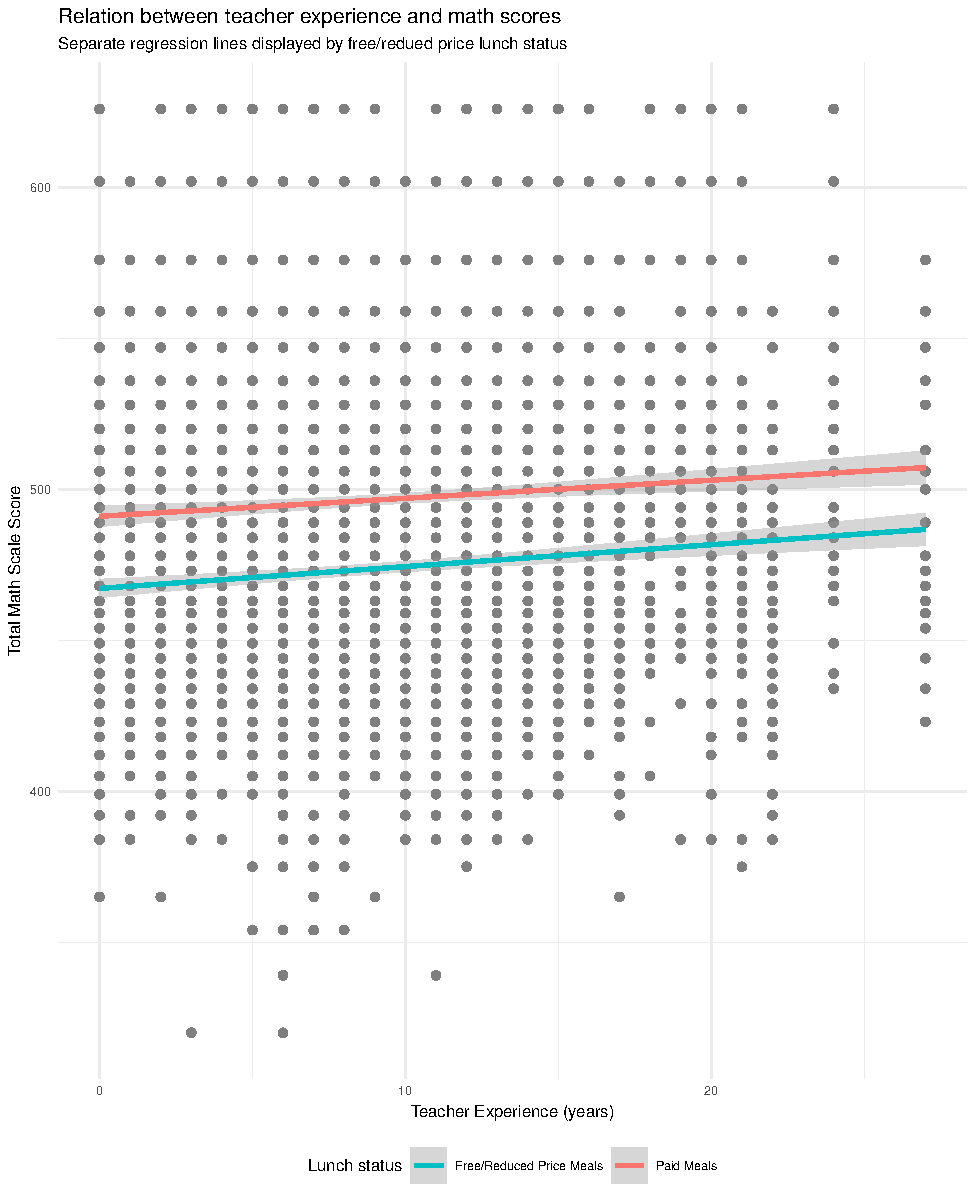
\includegraphics{Test_files/figure-latex/figure-1.pdf} According to the
figure, teachers' experience does not play an important role on
students' math performance but students' social economic status (SES)
does. Student with a lower SES status, indicated by having a
free/reduced lunch, has a lower math score compared to those who have
high SES status.

\section{Discussion}\label{discussion}

Vowel space is complex (see Logemann (1998)) Munro, Flege, and MacKay
(1996) reported that vowel space and language acquisition are closely
related

\newpage

\section{References}\label{references}

\begingroup
\setlength{\parindent}{-0.5in} \setlength{\leftskip}{0.5in}

\hypertarget{refs}{}
\hypertarget{ref-logemann1998evaluation}{}
Logemann, J. A. (1998). The evaluation and treatment of swallowing
disorders. \emph{Current Opinion in Otolaryngology \& Head and Neck
Surgery}, \emph{6}(6), 395--400.

\hypertarget{ref-munro1996effects}{}
Munro, M. J., Flege, J. E., \& MacKay, I. R. (1996). The effects of age
of second language learning on the production of english vowels.
\emph{Applied Psycholinguistics}, \emph{17}(3), 313--334.

\endgroup


\end{document}
